\documentclass{article}
\usepackage[utf8]{inputenc}
\usepackage{amsmath}
\usepackage{geometry}
\usepackage{graphicx}
\usepackage{hyperref}   

\title{Project - Interactive Graphic}
\author{Sveva Pepe - 1743997 \\ 
        Simone Tedeschi - matricola \\
        Claudia Medaglia - matricola \\
        Christiam Marinoni - matricola}
\date{}


\usepackage{listings}
\usepackage{xcolor}
\usepackage{geometry}
 \geometry{
 a4paper,
 total={170mm,257mm},
 left=25mm,
 top=25mm,
 right = 25mm,
 bottom = 25mm
 }
\definecolor{codegreen}{rgb}{0,0.6,0}
\definecolor{codegray}{rgb}{0.5,0.5,0.5}
\definecolor{codepurple}{rgb}{0.58,0,0.82}
\definecolor{backcolour}{rgb}{0.95,0.95,0.92}

\lstdefinestyle{mystyle}{
    backgroundcolor=\color{backcolour},   
    commentstyle=\color{codegreen},
    keywordstyle=\color{magenta},
    numberstyle=\tiny\color{codegray},
    stringstyle=\color{codepurple},
    basicstyle=\ttfamily\footnotesize,
    breakatwhitespace=false,         
    breaklines=true,                 
    captionpos=b,                    
    keepspaces=true,                 
    numbers=left,                    
    numbersep=5pt,                  
    showspaces=false,                
    showstringspaces=false,
    showtabs=false,                  
    tabsize=2
}
\lstset{style=mystyle}
\begin{document}
\maketitle
\section{Introduction}
The goal of the project is to implement an interactive application 
that make use of basic WebGL or advanced libraries, as in our case ThreeJS. The project 
cover the main aspects treat during the course, such as 
lights, textures, hierarchical models and animations.
\section{The Game}
We decided to develop a 3D version of "Duck Hunt", a  
famous game from the 80s, in which the objective is to hit  
as many ducks as possible. We designed the
scene as a first-person game, where the player is located 
in a tall grass field and controls a rifle. 
Thanks to the help of his dog, that frighten the ducks hidden 
in the tall grass, the hunt can start. 
The game ends when the player miss five ducks.
In addition, our game provides other functionalities like enable 
and disable sounds, pause the game or restart it.
\\ \\The above described scene is depicted in the following figure:
\begin{figure}[hbt!]
    \centering
    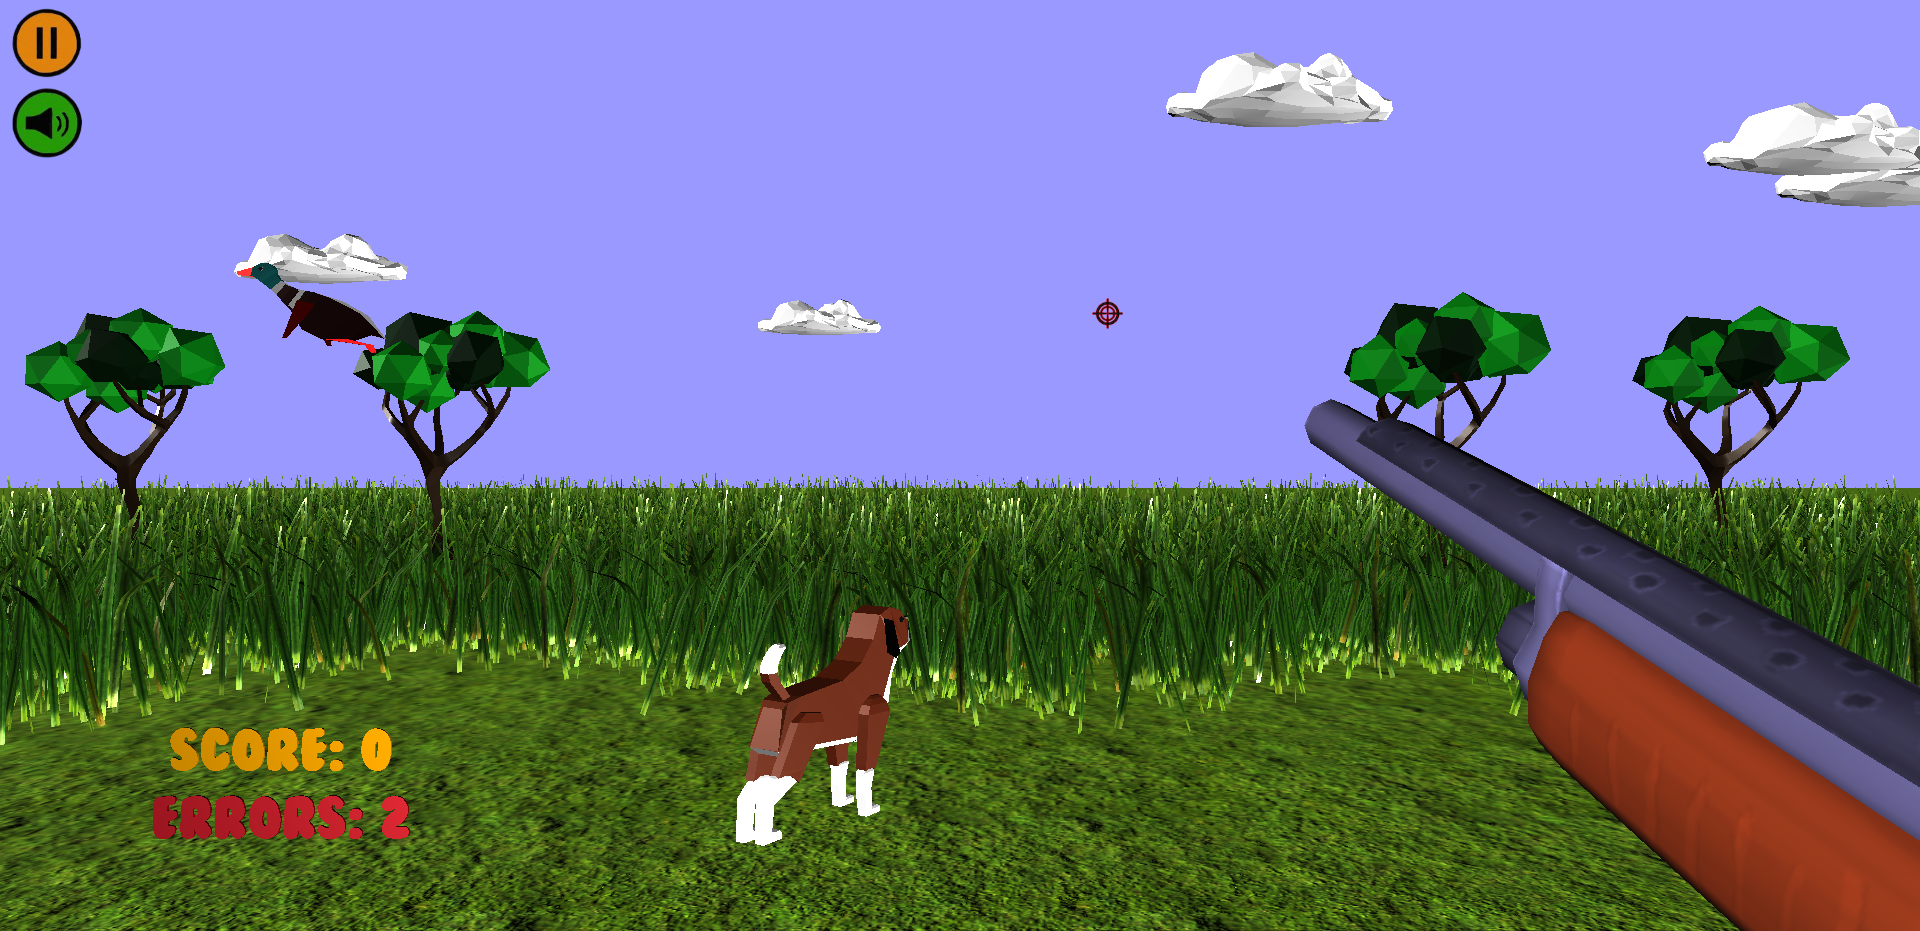
\includegraphics[width=0.8\textwidth]{game.png}
    \caption{Starting scene of the game.}
    \label{fig1}
\end{figure}
\section{The Scene}
The scene shown in Figure \ref{fig1}, which is a ThreeJS object, 
has been obtained adding textures, lights, and different 3D models. 
The dog and the ducks are hand-made models while the other are 
taken from SketchFab. We used perspective camera to make the scene 
as realistic as possible to let the center of projection coincide 
with the user’s eyes.
The prospective uses as parameters: \textit{fovy, aspect, near and 
far}. \textit{Fovy}, which stands for "field of view y-axis",
identifies how wide the eyes open along the y direction.
\textit{Aspect} represent the ratio between the width and height
of the canvas.
\textit{Near} and \textit{far} are any positive numbers 
representing the minimum and maximum distances of the object, 
with the restriction that near is always less than far.
For the camera is defined also the  
\textit{lookAt(x, y, z)} method, where the \textit{x, y} and \textit{z} 
are the coordinates of the scene.
The texts on the bottom right corner instead, have beed modeled using
TTFLoader of ThreeJS, where through a Mesh the relative 
colors have been applied.
Moreover, in order to make our application responsive we add a 
dedicated Listener to adapt the window size based on the device
resolution. Finally, to improve the user experience antialiasing 
has been used.
\subsection{Lights and Textures}
The ground texture was created by repeatedly applying a texture on 
a plane, using a TextureLoader. Then, the texture is added to the
scene through the use of meshes that map texture coordinates into
world coordinates.
Three directional lights have also been added to the scene. 
Two of them were placed on the left upper and bottom right corner 
respectively of the scene to reproduce a sunny day, otherwise using
only one of them we obtain either dark clouds or dark objects. 
The third one has been introduced to illuminate texts because they 
are ahead of other elements and so the previous lights were
not able to light up also them.
\section{3D Models}
The models we have included in our project can be divided into 
two categories: linear models, mainly models taken from sketchfab 
and hierarchical model, modeled for animations. 
\subsection{Linear Models} \label{linear}
\subsection{Hierarchical Models}
\section{Animations}
\section{User Interaction} \label{user}
\subsection{Sounds}
\section{Conclusion}
\end{document}